\documentclass[conference]{IEEEtran}
\IEEEoverridecommandlockouts
% The preceding line is only needed to identify funding in the first footnote. If that is unneeded, please comment it out.
\usepackage{cite}
\usepackage{amsmath,amssymb,amsfonts}
\usepackage{algorithmic}
\usepackage{graphicx}
\graphicspath{ {./images/} }
\usepackage{textcomp}
\usepackage{xcolor}
\def\BibTeX{{\rm B\kern-.05em{\sc i\kern-.025em b}\kern-.08em
    T\kern-.1667em\lower.7ex\hbox{E}\kern-.125emX}}
\begin{document}

\title{IDENTIFY THE PLANT AND DISEASE BASED ON THE LEAF PROVIDED\\
{\footnotesize Data Mining and Machine Learning II}
}

\author{\IEEEauthorblockN{Pedro Acosta}
\IEEEauthorblockA{\textit{School of Computing} \\
\textit{National College of Ireland}\\
Dublin, Ireland \\
x21138745@student.ncirl.ie}
\and
\IEEEauthorblockN{Brendan O’Dwyer}
\IEEEauthorblockA{\textit{School of Computing} \\
\textit{National College of Ireland}\\
Dublin, Ireland \\
x21145172@student.ncirl.ie}
\and
\IEEEauthorblockN{Femi Adeboye}
\IEEEauthorblockA{\textit{School of Computing} \\
\textit{National College of Ireland}\\
Dublin, Ireland \\
x21137684@student.ncirl.ie}
\and
\IEEEauthorblockN{Antonio Milian y Albacar}
\IEEEauthorblockA{\textit{School of Computing} \\
\textit{National College of Ireland}\\
Dublin, Ireland \\
x19172125@student.ncirl.ie}
}

\maketitle

\begin{abstract}
Detecting plant diseases at an early stage allows the implementation of plans to control their propagation, the current research offers a tangible solution that could be used by all types of farmers or gardeners outdoors regardless of the size of the business, harvest and natural outdoor conditions including surroundings. It is technical flexible as it could be implemented either in traditional mobile devices with cameras such as smartphones and tablets as well as in bigger and complex systems as an embedded module that could be integrated with modern pesticide systems. The current investigation evaluates if using CNN could help to create reliable and robust classification models in indoor, outdoor and mixed conditions. Particularly, outdoor conditions introduce naturally more complexity in image classification, besides, the lack of datasets available with outdoor images labelled adds an important limitation to the research. Those challenges were addressed by applying data augmentation techniques and transfer learning, and pre-trained model layers using convolutional layers were evaluated and compared. MobileNet v.2 was selected for having better accuracy and faster findings in terms of accuracy, the comparison between all datasets suggests that it is not worth training a model in a mixed dataset.
\end{abstract}

\begin{IEEEkeywords}
Convolutional Neural Networks, Plant Disease Detection, Adam, Hyperparameters Optimization 
\end{IEEEkeywords}

\section{Introduction}
Emerging technologies and diverse applications make it possible nowadays to detect early situations and conditions and hence prevent consequences that impact not only financially but in the life quality of people. Nowadays geopolitical conflicts urge all stakeholders in society to reduce errors and waste of resources, especially on food and all the chain, the current project aims to contribute and make possible the early detection through images of the type of plant and serves to early detect diseases on them. From small farmers that use their mobile phones to industrialized companies taking images with drones, the main objective is to make available the results and techniques from this study for them to be integrated or embedded as part of a simple, complex or wider solution that includes not only indoor analysis but also outdoor data. \

Since one of the core objectives of the project is to provide a reliable model that identifies plants diseases based on outdoor images, this scenario adds a level of complexity due to the nature of the situation, noise or information factors such as illumination, background, disease signs distributed randomly along with the different type of plants around, all contribute to the right application of the technique including modelling, hyperparameters optimization, among with some other methods required to work out any particular characteristics that datasets could have.  \

The research question is orientated to compare the performance of three classification models applying Convolutional Neural Network (CNN), the first model was trained with the PlantVillage dataset taken indoors, the second model was trained with the Plan Doc dataset taken outdoor images and the third dataset was trained with a combined dataset merging both previous datasets. Within the main objectives of this project is to address natural and technical challenges of the datasets, through experiments and results comparison, this research look to present the model with the  highest performance in terms of precision.  \

The current project is presented in 4 sections, related work included XX projects reviewed, the methodology discloses how images were pre-processed, how the techniques and methods were applied to generate each model, this included the comparison between two well-known convolutional layers used to transfer learning, everything applying CRISP-DM, it also includes  results included visual content with an analysis of each situation, finally, conclusions suggests relevant future works related to this research, natural limitations of the investigation and the implementation of additional techniques.  

\section{Related work}
Traditional machine learning methods require feature extraction, which is one of the most important and time-consuming steps. Convolution neural networks (CNNs) eliminate this step. Deep CNN models are still challenging to train using limited training data. The problem has been solved by using transfer learning and fine-tuning parameters. A trained model on a similar problem is modified to identify leaves by observing images in line with current trends. Deep learning can outperform traditional machine learning methods if the training sample size is small, according to the author of his study. Using transfer learning and parameter fine tuning, the author successfully trained an existing neural network using the latest trends in deep learning. An image recognition dataset, i.e., ImageClef2013 Plant Identification, was used to develop the CNN model, and it outperformed traditional machine learning methods. (15) 

According to the present study, the authors suggest exploiting an existing classifier and applying it to other seismic data using Transfer Learning techniques. Convolutional Neural Networks (CNNs) are optimized and trained on synthetic seismic data to form a base model. Results of Transfer Learning for the Netherlands offshore F3 block are presented. Even with a naturally high imbalance of the labeled classes as input, the method gives satisfactory results. This technique is suitable for practical use daily because it can be easily tuned and trained on a CPU in a few minutes. (12). There has been extensive interest in the current convolutional neural network approaches because they perform better than conventional machine learning methods in recognizing plant diseases. Despite this, challenges remain. It is sometimes difficult to use the model and detect specific pest positions because of complex image backgrounds. It is difficult to deploy and develop mobile software due to the complexity of the model. Disease recognition is restricted by errors in labeling, a small number of positive samples, and a limited number of negative samples, even in the dataset. Using deep transfer learning for plant disease recognition, deep convolution networks are investigated in this study. This paper proposes a model called Selective Kernel MobileNet (SK-MobileNet) that significantly reduces server computing costs. Results of the experimental study show that the proposed approach achieves an accuracy of 99.28%. With less complexity than other existing approaches, the proposed approach shows a significant improvement in efficiency. (22). 

All products have expiration dates. A product's recommended use period is represented by this indicator. However, keeping track of expiry dates can be difficult with many products to store. A transfer learning technique in deep learning is used in this work to solve the problem. The Convolutional Neural Network (CNN) - Inception ResNet V2 was trained on synthetic data containing images of near-realistic expiration dates. A synthetic image from Inception ResNet V2 was accurate to 0.9964, and a noisy image to 0.9612. Inception ResNet v2 was trained and deployed into the mobile application built to help users monitor expiration dates quickly and easily. A System Usability Scale (SUS) score of 85.7 was achieved in the usability test. The mobile application was well received by users. (7) Among the most common neurodevelopmental disorders, autism spectrum disorder (ASD) severely affects patients' daily lives and ability to interact socially. The correct therapeutic adaptations can be determined with an early and accurate diagnosis to allow patients to maintain a near-normal quality of life. It is highly subjective and time-consuming to diagnose ASD using current methods. As a popular solution today, functional magnetic resonance imaging (fMRI) is used to analyze abnormalities in brain functions. With the help of Inception v3, this study uses transfer learning to classify ASDs using fMRI data using a transfer learning-based approach. An epi, stat map, and glass brain image is created from a raw 4D fMRI dataset. Pre-trained weights improve classification accuracy. ASD can therefore be detected from fMRI images using pretrained ImageNet models incorporating transfer learning. Medical images can be analyzed using technology-enhanced decision support systems. The study has introduced a transfer learning-based approach to identify ASD using fMRI images. Medical image performance can be improved significantly using pre-train ImageNet models, according to the author. When trained with ImageNet weights, Inception v3 classified epi images 98% accurately. (9) 

An image classifier built using VGG - 16 with Deep Convolutional Neural Networks is used in this paper. Several neural network models were trained and validated in this study. A convolutional neural network-based model provides 72.40\% validation accuracy. An accuracy of 79.20\% was achieved by fine-tuning this model with image augmentation. As a last step, the author employed an existing model (VGG-16) which has been trained on a large dataset of images and fine-tuned using image augmentation to gain an accuracy of 95.40\%. (10) This article uses a CNN model trained for deep learning to extract facial features. Following the extraction of facial features, a DNN is trained for age range classification based on those features. Furthermore, CNN models previously trained for different tasks other than age range classification are dimensionally reduced in the last convolutional layer. A DNN architecture is used to incorporate and train dimensionally reduced features to estimate the age. The proposed method is demonstrated to be capable of estimating the age of an individual based on facial images through extensive experiments. Adience benchmark results were significantly outperformed by the proposed work by approximately 12\%. (11)  

Deep learning methods are used in the author's review of some recent approaches to colorizing grayscale images. InceptionResNet-v2 pre-trained model and a deep convolutional neural network are combined in this model, which is based on these findings. Using end-to-end deep learning architectures, this project validates that some image colorization tasks can be solved. As a result, high-level image components, such as the sky, the sea, or forests, can be colored successfully. Even so, there is still room to improve the quality of coloring intricate details. In this study, the author only used a subset of ImageNet; therefore, the ability of the algorithm to recognize unseen images depends on their specific content. A larger training dataset should be used to train the network to overcome this problem. (1) The study shows that captioning can yield plausible results using deep CNNs and a well-chosen objective function. It is still necessary to improve the ability to form and connect sentences properly. There are often partial errors in images caused by not paying attention to details (e.g., correcting a picture of a dog walking through the grass as a picture of a dog walking in an enclosure because bushes are in the background). Recent attention-mechanism studies suggest this task can be improved with attention-mechanisms. This study explores the effects of emitted words on hidden states in the LSTM, which is a novel contribution to this field. (3) Using convolutional neural networks, the author develops a model for detecting bridge cracks end-to-end. Convolution and residual networks are combined in this model, which broadens the network width and alleviates the deep network's training problem. While still ensuring accuracy, calculation speed has been improved. Multi-scale feature fusion allows the network to detect cracks with improved accuracy by extracting contextual information of different scales. A genetic algorithm-based K-means clustering method (GKA) performs accurate segmentation of a target area, maximizes clustering effects, and improves detection speeds. Training and testing are conducted with large fracture datasets without pre-training. In terms of accuracy, recall, F-measure, and frames per second, the experimental results identified a significant increase in the performance of this method: 99.24\%, 99.03, 99.79, and 196, respectively. (4) 

Several famous scenic spots have used face recognition technology in recent years. While the technology is useful for simplifying the ordering process for tickets, it is still difficult to use because fake ID cards are being obtained for purchasing tickets that do not match the genuine age categories. This paper proposes the use of face-based age recognition technology to improve the efficiency of ticket inspections by integrating it into ticket inspection. A simple convolutional neural network was replaced in this paper to fine-tune Inception ResnetV2 for recognizing facial features. Age recognition accuracy has improved significantly according to the experiment results.(5) The differences in some parts of the brain can be used to detect autism spectrum disorders (ASD). The author used the resting-state Functional Magnetic Resonance Imaging data provided by Autism Brain Imaging Data Exchange I (ABIDE I) and reorganized it into two-dimensional data to create a set of neuroimage data sets. Shear transformation, brightness adjustments, and zooming were performed on this dataset. The data was also resampled and normalized. Using only 2D neuroimages, this classification accuracy for autism should be improved based on past studies. InceptionResNetV2 was proposed to be used with the augmented dataset to utilize transfer learning. Training, validation, and testing results remained at 70.22\%, 57.75\%, and 57.6\%, respectively, after freezing layer by layer. Up to 2.6\% better performance was obtained with the transfer learning approach than with convolutional neural networks (CNN). (6)  

In conjunction with fine-tuning trained convolutional networks (Xception, Inception-Resnet, VGNets, Mobilenet, and Densenet), this study proposes a novel crop/weed identification system. As a result of the previously extracted features, the "traditional" machine learning classifiers (Support Vector Machines, XGBoost and Logistic Regression) were trained with the previously deep extracted features. This method avoided overfitting and ensured consistent performance without overfitting. Our approach was evaluated by generating unrestricted access datasets of two crops, tomato (Solanum lycopersicum L.) and cotton (Gossypium hirsutum L.), as well as weed species, black nightshade (Solanum nigrum L.) and velvetleaf (Abutilon theophrasti Medik.). Photos were captured at various production locations throughout Greece using RGB cameras under natural variable lighting. Based on the results, a fine-tuned Densenet and Support Vector Machine combination achieved a micro F1 score of 99.29\% with very minimal differences within the train and test sets. In other evaluations, over 95\% of F1 scores were obtained repeatedly. A heuristic for avoiding overfitting while not compromising performance is provided by their analysis of the results. (8) Increasing the number of hidden layers was not preferred in previous years due to calculation complexity. Since GPU technology allows calculations to be performed more quickly, deep learning has once again gained popularity. For the classification of large-scale images, Convolutional Neural Networks (CNN) are used in deep learning models. Among deep learning models, CNN is most used for learning features, recognizing them, and classifying them. We are attempting to classify gender in this study. New CNN models have been designed to achieve this goal. This CNN model was trained and tested using the Adience data set. According to the experiments, 88.5\% of gender classifications were accurate. Comparing the proposed model to machine learning methods and other CNN models, it has been found to obtain the best accuracy value. (13)  

For lung nodule detection and classification, massive-training artificial neural networks (MTANNs) and convolutional neural networks (CNNs) are used as dominant end-to-end learning machines. CNNs have recently gained popularity in the field of medical imaging, despite MTANNs having been active for two decades. The purpose of this study is to compare both experimentally and theoretically these two successful learning machines. To achieve this goal, we examined two well-studied topics in medical image analysis: detecting lung nodules in computed tomography (CT) and distinguishing benign from malignant nodules. To perform a comprehensive analysis, the author used two optimized MTANN architectures and four distinct CNN architectures. With limited training data, MTANNs performed significantly better than CNNs. Although the performance gap remained significant, it became less apparent with a larger training dataset. At 100\% sensitivity, MTANNs generated significantly fewer false positives per patient than the best performing CNN model which generated 22.7 false positives per patient. The AUC of MTANNs was 0.8806 (95\% CI: 0.8389–0.9223), a significant improvement over the CNN model's AUC of 0.7755 (95\% CI: 0.7120–0.8270). Thus, MTANNs would be a good machine-learning model for detecting and classifying focal lesions with limited training data. (14) This paper evaluates four different deep learning models with machine learning algorithms and proposes and implements four different deep learning models. When compared to other deep learning algorithms and machine learning algorithms, the hybrid CNN+LSTM model performed better with 97.16 percent accuracy. In addition, the MLP deep learning model provides the least performance on the dataset. Based on the results, all three deep learning methods perform better than machine learning algorithms, except for MLP, which gets more than 95.00\% accuracy. (16) DLNNs were introduced as a model to assess landslide susceptibility and their predictive performance compared to existing machine learning methods. When comparing the results of the DLNN model with MLP-NN, SVM, C4.5, and RF models, it outperformed all of them. The classification performance of neural network-based models was more stable than that of tree-based models. Classification accuracy, sensitivity, specificity, and area under the success curve (AUC) of each model were calculated as a method of evaluating its learning and predictive potential. A comparison of the proposed DLNN model with four benchmark models showed that it had a higher performance. It was found that deep learning approaches can be considered as satisfying alternatives for landslide susceptibility mapping, although it has been rarely used in landslide susceptibility assessments. (17) 

Automatic disease detection models that use deep learning exhibit mediocre performance when applied to real world images that are unfamiliar. This study shows that segmented and annotated images can be used instead of full images to train a convolutional neural network (CNN). The performance of CNN models on independent data increases from 42.3\% to 98.6\% when trained on segmented images (S-CNN) rather than full images (F-CNN). Moreover, 82\% of the test dataset showed improved self-classification confidence, according to quantitative analysis. It will be increasingly important to pre-process images before CNN training as better data sets become available soon. (19) An architecture for detecting plant leaf diseases using Convolutional Neural Networks (CNNs) is presented in this paper. Based on 54,305 images of both healthy and unhealthy leaves from the Plant Village Dataset, a CNN model is trained. The proposed architecture achieves a disease classification accuracy of 95.81\%, and various observations have been made with different CNN hyperparameters. (20) Among the most important vegetables in the world, tomatoes have a significant economic impact. It is notoriously difficult to eliminate completely viral diseases against plants, despite tremendous efforts in plant management. Therefore, early detection of plant diseases is necessary to mitigate the problem. Using computer vision, leaf images are captured, and the possibility of diseases detected. The decision is made using an artificial deep learning classifier that can handle a wide range of leaf appearances. Three types of tomato diseases have been detected with MobileNet V2, a compact deep learning architecture. A total of 4,671 images from the PlantVillage dataset were used to test the algorithm. According to the study, more than 90\% of the disease can be detected with MobileNet V2. (21) 

There has been extensive interest in the current convolutional neural network approaches because they perform better than conventional machine learning methods in recognizing plant diseases. Despite this, challenges remain. It is sometimes difficult to use the model and detect specific pest positions because of complex image backgrounds. It is difficult to deploy and develop mobile software due to the complexity of the model. Disease recognition is restricted by errors in labeling, a small number of positive samples, and a limited number of negative samples, even in the dataset. Using deep transfer learning for plant disease recognition, deep convolution networks are investigated in this study. This paper proposes a model called Selective Kernel MobileNet (SK-MobileNet) that significantly reduces server computing costs. Results of the experimental study show that the proposed approach achieves an accuracy of 99.28\%. With less complexity than other existing approaches, the proposed approach shows a significant improvement in efficiency. (22) This paper presents a method for identifying cash crop diseases by combining automatic image segmentation with deep learning. AISA removes the background information from images, but retains the disease spots, using the GrabCut algorithm. Several crop images from the Internet and practical planting bases are added to the public dataset PlantVillage to increase MobileNet's generalization ability. The MobileNet Convolutional Neural Network (CNN) model was selected as the deep learning model. To extract disease features from crop leaf images, the AISA processes them first, resulting in significant reductions in calculations. Using the system in this paper, the author estimates it correctly recognizes 27 diseases in 6 crops with a correct recognition rate of more than 80\% and has a high application value. (24) 

A two-step comparative evaluation of plant disease has been proposed based on deep learning in this study. An analysis of popular CNN architectures in addition to enhanced and hybridized versions of some of the Deep Learning models developed in recent studies were investigated to determine the best CNN. As a second step, various deep learning optimizers were used to improve the performance of the best-obtained model. Several performance metrics were compared between various CNNs, such as the validation accuracy/loss, the F1-score, and the number of epochs. Deep learning architectures were trained using Keras and TensorFlow. Using the Adam optimizer, the Xception architecture was able to achieve 99.81\% validation accuracy and 0.9978 F1 score, which are significantly higher than the previous approaches and demonstrate its novelty. It is consequently possible to apply the method proposed in this study to other agricultural applications for the purpose of accurate detection and classification of agricultural products. (23  

\section{Methodology }

The Cross Industry Standard Process for Data Mining (CRISP-DM) data mining methodology has been followed in this study. The data mining lifecycle is described by the five phases of this methodology. It is a flexible and iterative process. Phases can be revisited as the project progresses. This study will involve training different models and as a result phases will be revisited repeatedly. Business understanding is the first phase in CRISP-DM. The data mining goals are determined in this phase and an understanding of the objectives and requirements of the project developed. In the introduction the objectives of the study have been outlined. The business understanding phase is addressed through these objectives as well as through the understanding developed from the related work publications. In the remainder of this report a description of the other CRISP-DM phases is provided.
\begin{figure}[htbp]
\centerline{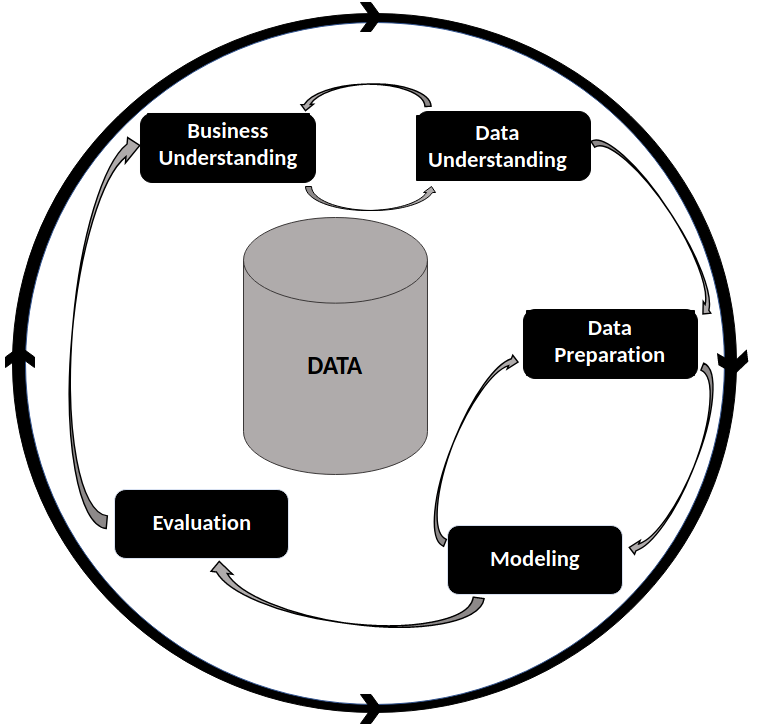
\includegraphics[width=8.5cm]{CRISP_DM_no deployment.png}}
\caption{    The phases of the CRISP-DM cycle. Business understanding, data understanding, data preparation, modelling and evaluation in this case there is not deployment phase as the evaluation is the output.}
\label{fig}
\end{figure}



\subsection{Data Understanding}\label{AA}
Exploration and collection of data is carried out in the CRISP-DM data understanding phase. An understanding of the data is obtained as well as an understanding of how the objectives can be addressed through the data. Two datasets are used in this study. The first, PlantVillage \cite{kaggledatasetPlantville}, contains labelled images with diseased and healthy plant leaves. The images are taken indoors in laboratory conditions. The data are made available through the PlantVillage online platform. In total there are over 50,000 images of crop plant leaves that are infected or healthy. There are 14 different types of plant species with 38 classes in total. Each class corresponds to a plant-disease pair. 

The second dataset, Plant Doc\cite{kaggledatasetPlantDoc}, is for detecting plant disease from images. Unlike the first dataset the images are taken outdoors rather than in laboratory conditions. There are 2,598 images in total with 13 species of plants in total with 17 disease classes. The data were obtained by scraping images from webpages and annotating them. 

The PlantVillage dataset contains coloured, segmented and greyscale versions of each image. The coloured versions of the images were used. In the case of Plant Doc only colour images are provided. This study used 13 classes with 18,317 images from both datasets, PlantVillage and Plant Doc.  
\subsection{Data Preparation}
This phase of CRISP-DM involves manipulating data acquired in the data understanding phase to prepare it for the modelling phase. The datasets were explored using Python. The feature selection is based on the commonalities between the previously described datasets. \

Three plant species present in both the PlantVillage and Plant Doc datasets were selected apple, pepper and tomato. In total there are 13 disease classes for these plants common to both datasets. These classes are apple scab leaf, apple healthy leaf, apple rust leaf, bell pepper leaf healthy, bell pepper leaf spot, tomato early blight leaf, tomato septoria leaf spot, tomato leaf healthy, tomato leaf bacterial spot, tomato leaf late blight, tomato leaf mosaic virus, tomato leaf yellow virus and tomato mold leaf, more details for the classes in Table I. 
\begin{table}[htbp]
\caption{Data Sets used}
\begin{center}
\begin{tabular}{|c|c|c|c|c|}
\hline
\textbf{Classes}&\multicolumn{4}{|c|}{\textbf{Data sets}} \\
\cline{2-5} 
\textbf{Ojbective} & \textbf{\textit{Indoor}}& \textbf{\textit{Outdoor}}& \textbf{\textit{O.Augmented}} & \textbf{\textit{Combined}} \\
\hline
apple scab &630&87&1307&1937 \\
\hline
apple healthy &275&89&1392&1667\\
\hline
apple rust &1645&91&1325&2970\\
\hline
bell pepper healthy &997&71&1355&2352\\
\hline
bell pepper spot &1478&61&1581&3059\\
\hline
tomato early blight &2127&107&1256&3383\\
\hline
tomato septoria  &1591&62&1392&2983\\
\hline
tomato healthy &1000&83&1379&2379\\
\hline
tomato bacterial &1771&148&1272&3043\\
\hline
tomato late blight &1909&111&1306&3215\\
\hline
tomato mosaic  &373&54&1131&1504\\
\hline
tomato yellow virus &5357&75&1172&6529\\
\hline
tomato mold &952&91&1444&2396\\
\hline
\multicolumn{5}{l}{$^{\mathrm{a}}$Original Data set classes and values.}
\end{tabular}
\label{tab1}
\end{center}
\end{table}

Two test datasets were created. The first uses only images from the dataset of indoor laboratory data. The second consists of images taken outdoors from the Plant Doc dataset. For each of the PlantVillage and Plant Doc datasets the remaining data are assigned randomly to training datasets, validation datasets and datasets used for tuning hyperparameters. 72\% of the data are assigned to the training datasets, 20\% are assigned to the validation datasets and 8\% are assigned to the datasets for tuning hyperparameters. \

All images were adjusted to have the dimensions 240 pixels by 240 pixels for InceptionResNetv.2 and to 224 x224 when using MobileNetv.2. The PlantVillage dataset has more images for each class than the Plant Doc dataset. As a result of this data augmentation techniques were applied to the Plant Doc dataset. These techniques included rotation, shearing, zooming, flipping horizontally and adjusting the brightness range. The data was pre-processed. The pixel values are rescaled. 
\subsection{Modelling}
CNN was the model typology used to analyse the data and take advantage of the properties of the models in image recognition, Modelling techniques are used to build and assess models in the CRISP-DM modelling phase. A batch size of 32 was used. As convolutional layers two types are taken into consideration, Inception ResNet, in this case the pre-trained convolutional neural network and Inception-ResNet-v2 was used for transfer learning. Weights trained on the ImageNet dataset, which has one thousand classes and 1.4 million images, were used. On top of this model, a new classifier is added. The layers of the base convolutional model are frozen. The second type is MobileNet. In addition to Inception-ResNet-v2 the pretrained convolutional neural network MobileNet V2 was also used for transfer learning. The data were again preprocessed in preparation for use with the MobileNet V2 model. Weights trained on the ImageNet dataset were used. As before a new classifier was added on top of this model and the layers of the base convolutional model were frozen. 
\subsection{Hyperparameter Optimisation}
Adding to the convolutional layers described the optimizers Adam and Adagrad were also tested. Combining the different values of convolutional layers and optimizers several models are proposed as potential candidates. The models are passed to a build model function in which several parameters are proposed for the rate of drop on the and the learning rate. A few values are provided for both variables. The optimization is centered in finding the best values for drop rate and from the learning rate. The model with the Convolution layer is frozen and a range of values proposed for both variables. The values for learning rates ranging from 0.01 to 0.00001, and the drop rates used range from 0.1 to 0.2. From the algorithm point of view, the library keras tuner has been used to ascertain the optimal values. From keras tuner, the Hyperband tuning algorithm is chosen. The algorithm has the championship bracket approach, running the models and choosing only the half best performers to be carried onto the next epoch.  This approach is faster and guarantees better results than a simple Grid optimization approach.  The keras tuner implementation has been run for 6 epochs in each trial, obtaining the optimal learning rate for each model as well as the optimal number of epochs.  Accuracy over the validation is the metric used to find the best parameter values. The goal is to decide which model’s architecture render the best validation accuracy and continue with that model through the fine-tuning process.\ 

Same methodology has been used for the three different implementations; the values gathered have subsequently used in the tested models. The three models were trained using the three different data sets, Indoors, Outdoor and Combined. The outdoor model is using the Outdoor data set, with the augmentation images for training.\ 

Applying the Hyperparameter optimization over the datasets the below results are obtained, 

\subsection{Model using the Indoor images}
Applying the Hyperparameter tuning to the indoor data set, the model that offers the best results has a convolutional layer based on MobileNet v.2 with the Adam optimizer, which gives not only better accuracy at 96.9\% but is also 4 times faster than the ResNet v.2 (94.5\%) with the same optimizer. Trying Adagrad as optimizer for MobileNet v.2  the accuracy obtained 95\%, so the model chosen for the indoor data set is MobileNet v.2 with Adam optimizer with the parameters obtained from the hyperparameter tuner. \

The images are transformed into 224 x 224 pixels, to match with MobileNet requirements. The drop rate is of 0.2 and the learning rate 0.0001 as provided by the Keras tuner algorithm. The dense layer has 1280 nodes and 16,653 trainable parameters. \
\begin{figure}[htbp]
\centerline{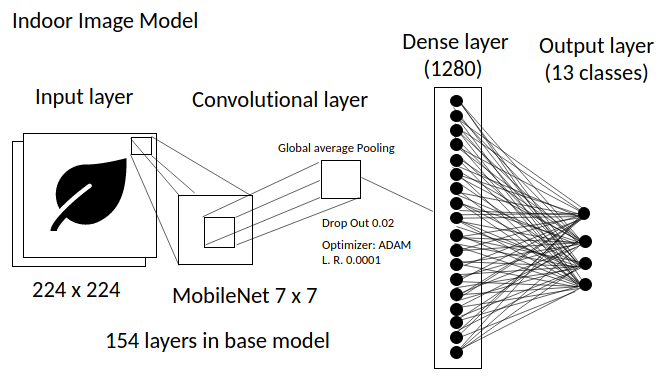
\includegraphics[width=8.5cm]{ModelIndoorsMobileNet.png}}
\caption{MobileNet Indoor model schema.}
\label{fig}
\end{figure}
The model is then trained for ten epochs before fine tuning. The accuracy obtained was 91.91\% for the training subset and 92.82\% for the validation subset as show in figure 3. The model was trained for another ten epochs for fine tuning. For fine tuning as series of modifications were introduced, the learning rate was reduced by a factor of 10 and the layers from 100 upwards were used in fine-tuning the model. For this model the total number of parameters was again 2,274,637, but in this case 1,878,093 of these were trainable. e fine tuning epochs a big increase on the accuracy is observed, where on the epoch 17 the accuracy of the validation reaches its maximum and the one from the training subset are similar at 98.55\%. For reference, in \cite{saleem2020plant} for classification of crop disease the authors carry out a comparison of deep learning architectures and optimisers. The best classification accuracy for the validation set was 99.81\% obtained using the Adam optimiser to train the Xception architecture.  
    
\begin{figure}[htbp]
\centerline{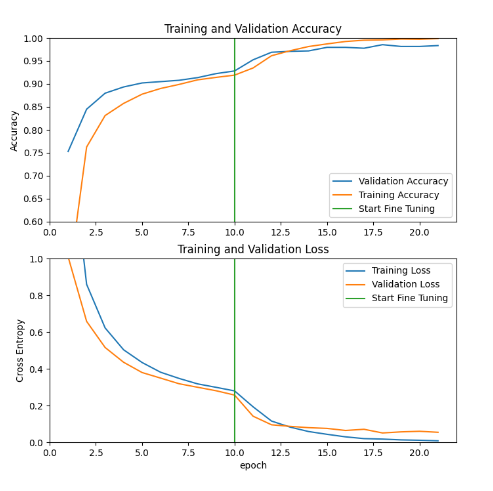
\includegraphics[width=8.5cm]{ModelIndoorsMobileNetEpochsAccuracychart.png}}
\caption{Model MobileNet v.2 with Adam Optimizer Indoor dataset for Accuracy and Cross Entropy.}
\label{fig}
\end{figure}
Similar behaviour can be observed using the metrics Precision and Recall, when around the 16 or 17 epoch the validation and training subsets provide the best outcome values. 


For this model the total number of parameters was again 2,274,637, but in this case 1,878,093 of these were trainable. e fine tuning epochs a big increase on the accuracy is observed, where on the epoch 12 the accuracy of the validation and the one from the training subset are similar at 97.4\%. For reference, in\cite{saleem2020plant} for classification of crop disease the authors carry out a comparison of deep learning architectures and optimisers. The best classification accuracy for the validation set was 99.81\% obtained using the Adam optimiser to train the Xception architecture. \
Similar behaviour can be observed using the metrics Precision and Recall, when around the 11 or 12 epoch the validation and training subsets provide similar values. 

\subsection{Model using the Outdoor images}
%A convolutional neural network model was trained on the PlantVillage indoor laboratory images and tested on both the test dataset of indoor images and the test dataset of outdoor images. Another CNN model was trained on the Plant Doc outdoor images and tested on both the indoor and outdoor test datasets. The indoor laboratory images and outdoor images were merged into a combined training dataset and a model was trained on this dataset and tested on both the indoor and outdoor test datasets. An additional model was trained on the augmented Plant Doc outdoor images dataset and tested on both test datasets. The augmented outdoor images dataset was merged with the indoor laboratory images dataset and a model trained on the combined dataset and tested on both test datasets. (to edit)

Applying the Hyperparameter tuning to the outdoor data set, the model that offers the best results uses the pretrained convolutional neural network MobileNet v.2 with the Adam optimiser, which gives not only better accuracy at 89.7% but is also 4 times faster than the ResNet v.2 (82.8%) with the same optimiser. Trying Adagrad as the optimiser for MobileNet v.2 the accuracy obtained is 83.3%, so the model chosen for the outdoor data set is MobileNet v.2 with Adam optimiser with the parameters obtained from the hyperparameter tuner. 

The images are transformed into 224 x 224 pixels, to match with MobileNet requirements. The drop rate is of 0.1 and the learning rate is 10-5 as provided by the Keras tuner algorithm. The dense layer has 1280 nodes and 16,653 trainable parameters. 

The model is then trained for ten epochs before fine tuning. The accuracy obtained was 40.9\% for the training subset and 45.2\% for the validation subset as shown in Figure x. The model was trained for another ten epochs for fine tuning. For fine tuning a series of modifications were introduced. The learning rate was reduced by a factor of 10. As the model we are training is much larger we reduce the learning rate. Our model may overfit quickly if at this stage we don’t adjust the learning rate. The layers from 100 upwards were used in fine-tuning the model. For this model the total number of parameters was again 2,274,637, but in this case 1,878,093 of these were trainable. In the fine-tuning epochs, a big increase on the accuracy is observed, where on the epoch 13 the accuracy of the validation and the one from the training subset are similar. The best validation accuracy obtained was 97.9%.  
\begin{figure}[htbp]
\centerline{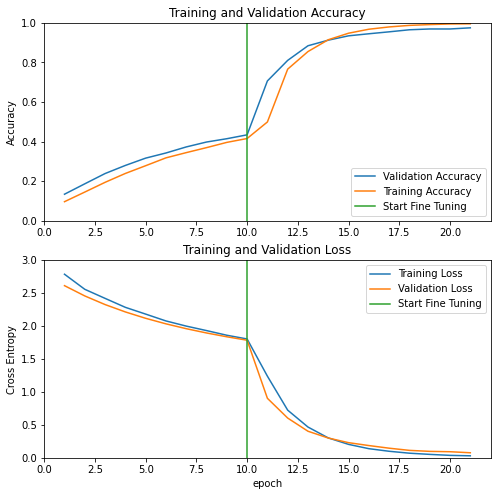
\includegraphics[width=8.5cm]{ModelOutdoorsMobileNetEpochsAccuracychart_new.png}}
\caption{For model trained on the augmented Plant Doc outdoor data with transfer learning using the pretrained MobileNet V2 CNN with fine tuning and Adam optimiser training and validation accuracy are plotted against epoch number in the upper panel. In the lower panel the training and validation loss are plotted against epoch number.}
\label{fig}
\end{figure}

Similar behaviour can be observed using the metrics precision and recall, when around epoch 13 the validation and training subsets provide similar values.
 
\begin{figure}[htbp]
\centerline{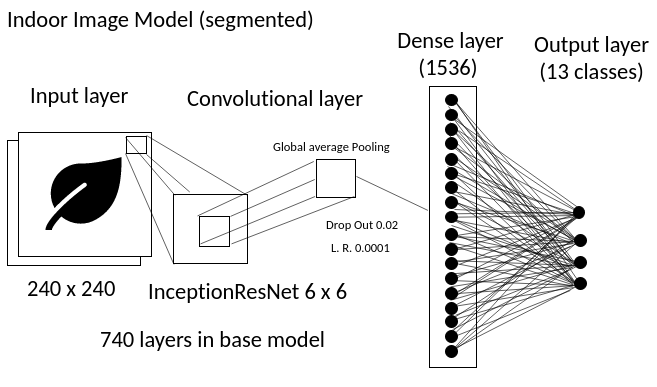
\includegraphics[width=8.5cm]{ModelIndoorsResNet.png}}
\caption{InceptionResNetv.2 Indoor Segmented model schema.}
\label{fig}
\end{figure}

\subsection{Combined data model}

The same methodology is applied to a dataset that combines the pictures from the outdoor and indoor data sets. The outdoor data includes the augmented added items in the training subset. From the data set thus conformed, a training data set of 33394 images is extracted and further divided into 30052 for the training side and 3339 for the validation. Using these images to compare the different models proposed, InceptionResNetV2 with Adam as optimizer, renders the best accuracy at 6 epochs for the optimized values of 0.1 drop and 0.00001 learning rate of 85.56\%. MobileNet with Adagrad  for the same number of epochs and optimized parameters, Learning Rate, 0.01 and drop, 0.1 renders better accuracy at 87.24\%. The best accuracy is obtained using the MobileNet with Adam, with the optimised values of 0.0001 for the learning rate and 0.2 for the drop at 90.35\%. It is also worth to acknowledge that the MobileNet instances were 4 times faster than the InceptionResNetV2, which would make them more compelling even with similar results. 

Using the best model from the hyperparameter tunning phase, it is trained for 10 epochs in a first phase where the layers are frozen for training, therefore only the parameters after the dense layer are trainable, 16,653 in total. The accuracy obtained is 79.19\% for the training set and 80.20\% for the validation set.  \

. \
\begin{figure}[htbp]
\centerline{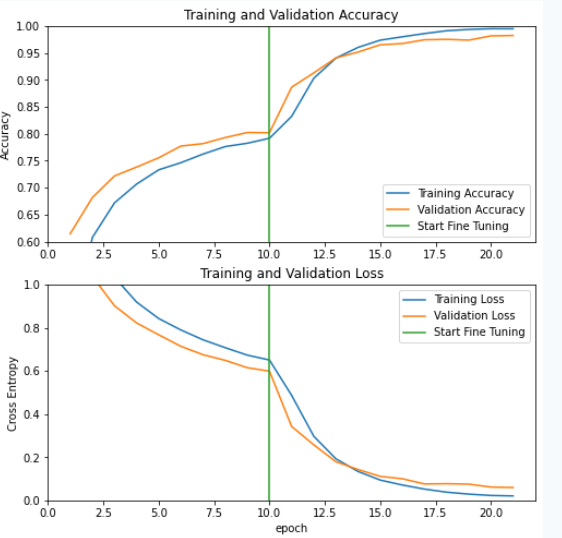
\includegraphics[width=8.5cm]{ModelCombineAccCEntropy.png}}
\caption{Model MobileNet v.2 with Adam Optimizer Combined dataset for Accuracy and Cross Entropy.}
\label{fig}
\end{figure}

After the first training phase is over, some of the layers of the convolutional part are made trainable, in this case 100 of them are kept frozen and 56 are deemed trainable, bringing the number of trainable parameters up to 1,878,093. During the fine-tuning phase, a great improvement can be observed in all metrics analyzed, up to the 14 epochs when the results of the validation subset go under the training ones, but the validation accuracy keeps growing up to 19th epoch when a validation accuracy of 98.16\% occurs. 

\subsection{Indoor Segmented dataset}
 

The performance of models trained with segmented images and the original unsegmented version of the same images was compared. For the PlantVillage indoor laboratory dataset a model was trained on the original unsegmented version of the images using transfer learning with Inception-ResNet-v2. The model was trained for ten epochs before fine tuning. The test accuracy obtained was 94.38\%. The model was trained for another ten epochs with fine tuning. The test accuracy obtained was 98.37\%. Another model was trained on the segmented version of the same images using transfer learning with Inception-ResNet-v2. The model was trained for ten epochs before fine tuning. The test accuracy obtained was 92.50\%.\
 The model was trained for another ten epochs with fine tuning. The test accuracy obtained was 96.88\%. The model trained on the original unsegmented data gave better test accuracy. In \cite{mohanty2016using} for the PlantVillage dataset experiments are run on the segmented leaves. Segmentation removes any background information. In their experiments models trained with segmented images are found to give worse performance than those trained with the original unsegmented images. While we are using a pretrained model for transfer learning which is different from the pretrained models in their work our results are consistent with models trained on the original unsegmented images giving better performance. It is possible that some inherent bias is introduced into the dataset due to the background information.   \ 

\begin{figure}[htbp]
\centerline{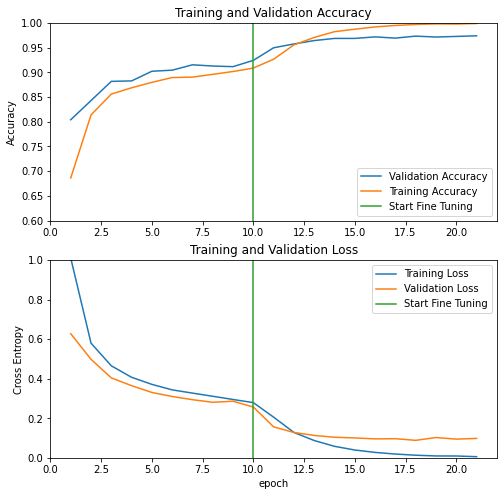
\includegraphics[width=8.5cm]{ModelIndoorsResNetEpochsSegmentedAccuracychart_new.png}}
\caption{For model trained on the PlantVillage indoor laboratory data segmented images with transfer learning using the pretrained Inception-ResNet-v2 CNN with fine tuning training and validation accuracy are plotted against epoch number in the upper panel. In the lower panel the training and validation loss are plotted against epoch number.}
\label{fig}
\end{figure}
 

\section{Results and Evaluation}


\subsection{Metrics used} 

To evaluate the performance of the proposed models the metrics to be used are accuracy, loss, precision, recall and area under the receiver operating characteristic curve (AUC).  Tensorflow provide a series of metrics tthat can be extracted from the model, 
\begin{itemize}
\item[•]Accuracy is defined as the number of samples that the model labels correctly divided by the total number of samples, it gives general idea of the total performance of the model, values closer to 1 are expected for models performing well. 
\item[•]Loss, the loss function used on the models is categorical cross entropy. It is defined by the below equation, 
\begin{equation} Loss = -\sum _{i=1}^{n}y_{i}-\log\hat{y_{i}} \end{equation} 
because $\hat{y_{i}} $ is one when the event is predicted multiplication provides a 0 value therefore lower values are expected from better models, where the predictions are right. 
\item[•]Precision calculates the ratio of the true positives by all positives across all classes as this is not a binary problem, it is defined as follows, 
\begin{equation} Precision= \frac{\sum _{c=1}^{Classes}TP_{c} }{\sum _{c=1}^{Classes}(TP_{c}+FP_{c})} \end{equation}  
it is also a value that ranges from 0 to 1 and the strongest model should provide a value closer to 1. 
\item[•]Recall is the ratio of the true positives in each class by the true positives and false negatives, defined below,  
\begin{equation} Recall= \frac{\sum _{c=1}^{Classes}TP_{c}}{\sum _{c=1}^{Classes}(TP_{c}+FN _{c})} \end{equation}  
A stronger model should show a value closer to 0. 
\item[•]AUC, the area under receiver operating characteristic (ROC) curve, the ROC plots the True positives rate (in y axis) with the False Positive Rate (in the x axis), intuitively, if the ratios are the same the ROC is the bisectrix of the first quadrant, and the AUC is 0.5, in the best case the True Positive ratios are much better than the false ratios, so the ROC curve bends towards the y axis given a AUC closer to 1. Bette performing models are expected to have an AUC value close to 1.
\end{itemize}\

The results shown in table III come from the model previously defined in methodology section Model Indoor dataset. The model has been trained for 17 epochs in total, 10 where only the dense layer was trainable and 7 more epochs with 54 layers more trainable and a learning rate reduced by a factor of ten. The model performs satisfactory over the Indoor test subset producing accuracy over 98.1\%, almost as good as the one produced by the validation subset in the model selection phase (98.5\%).   

\begin{table}[htbp]
\caption{Indoor Model}
\begin{center}
\begin{tabular}{|c|c|c|c|c|}
\hline
\textbf{Metrics}&\multicolumn{2}{|c|}{\textbf{Indoor Model}} \\
\cline{2-3} 
\textbf{Used} & \textbf{\textit{Indoor}}& \textbf{\textit{Outdoor}} \\
\hline
loss &0.058&9.788  \\
\hline
accuracy &0.981&0.075 \\
\hline
precision &0.982&0.083 \\
\hline
recall &0.978&0.075 \\
\hline
auc &0.999&0.537  \\
\hline
\multicolumn{3}{l}{$^{\mathrm{a}}$Over Indoor test and Outdoor test subsets.}
\end{tabular}
\label{tab1}
\end{center}
\end{table}
The model has been used over test Outdoor subset for purely comparative purposes and there is not any expectation in terms of performance in this instance.

Included in Table III for the model trained on the augmented outdoor data with MobileNet and the Adam optimiser for 14 epochs are evaluation metrics obtained by applying the model to the outdoor test set and the indoor test set. The training accuracy and validation accuracy values for epoch 14 were 91.46\% and 91.28\% respectively. After epoch 14 the model starts to overfit the training data. From Table x it can be seen that the accuracy obtained on the indoor test set is 23.27\%, higher than the accuracy obtained on the outdoor test set 9.17\%. The precision, recall and AUC values for the indoor test set at 0.2779, 0.1945 and 0.6798 respectively are also higher than the precision, recall and AUC values for the outdoor test set at  0.1087, 0.0833 and 0.5952 respectively.\
 


\begin{table}[htbp]
\caption{Outdoor Model}
\begin{center}
\begin{tabular}{|c|c|c|c|c|}
\hline
\textbf{Metrics}&\multicolumn{2}{|c|}{\textbf{Outdoor Model}} \\
\cline{2-3} 
\textbf{Used} & \textbf{\textit{Indoor}}& \textbf{\textit{Outdoor}} \\
\hline
loss  &4.92 &3.70  \\
\hline
accuracy  &0.0917 &0.2327 \\
\hline
precision  &0.1087 &0.2779 \\
\hline
recall  &0.0833 &0.1945 \\
\hline
auc  &0.5952 &0.6798  \\
\hline
\multicolumn{3}{l}{$^{\mathrm{a}}$For the model trained on the augmented outdoor data.}
\end{tabular}
\label{tab1}
\end{center}
\end{table}

The model has been trained for 19 epochs, 10 with the training layer being only the dense layer and a learning rate of 0.001 and for 9 epochs on the fine-tuning phase, meaning that has 56 training layers, the ones in the dense layer plus 54 from the convolutional layers. The model produced is applied then to both testing subsets, one from the indoor model that contains 4026 samples and another from the outdoor subset that contains 120 items. \
There is a superior performance when the test in conducted over the indoor test subset, at 98\% virtually the same precision and a recall of 97.3\%. The area under the curve is almost total at 99.9\%. Comparing this outstanding performance with the performance achieved with the outdoor test subset, with accuracy and recall at 9.2\%, precision 9.8\%, the area under the curve at slightly over the half bring to two conclusions. First, that the performance in outdoor subset is basically what it can be achieved randomly, taking into consideration that there are 13 classes of. Second, that the performance is not improving by including more images in the training set. \

\begin{table}[htbp]
\caption{Combined Model}
\begin{center}
\begin{tabular}{|c|c|c|c|c|}
\hline
\textbf{Metrics}&\multicolumn{2}{|c|}{\textbf{Combined Model}} \\
\cline{2-3} 
\textbf{Used} & \textbf{\textit{Indoor}}& \textbf{\textit{Outdoor}} \\
\hline
loss   &0.066 &9.024   \\
\hline
accuracy   &0.98 &0.092  \\
\hline
precision   &0.979 &0.098 \\
\hline
recall   &0.973 &0.092 \\
\hline
auc   &0.999 &0.542   \\
\hline
\multicolumn{3}{l}{$^{\mathrm{a}}$Over Indoor test and Outdoor test subsets..}
\end{tabular}
\label{tab1}
\end{center}
\end{table}

There is a superior performance when the test in conducted over the indoor test subset, at 98\% virtually the same precision and a recall of 97.3\%. The area under the curve is almost total at 99.9\%. Comparing this outstanding performance with the performance achieved with the outdoor test subset, with accuracy and recall at 9.2\%, precision 9.8\%, the area under the curve at slightly over the half bring to two conclusions. First, that the performance in outdoor subset is basically what it can be achieved randomly, taking into consideration that there are 13 classes of. Second, that the performance is not improving by including more images in the training set. 



\begin{figure}[htbp]
\centerline{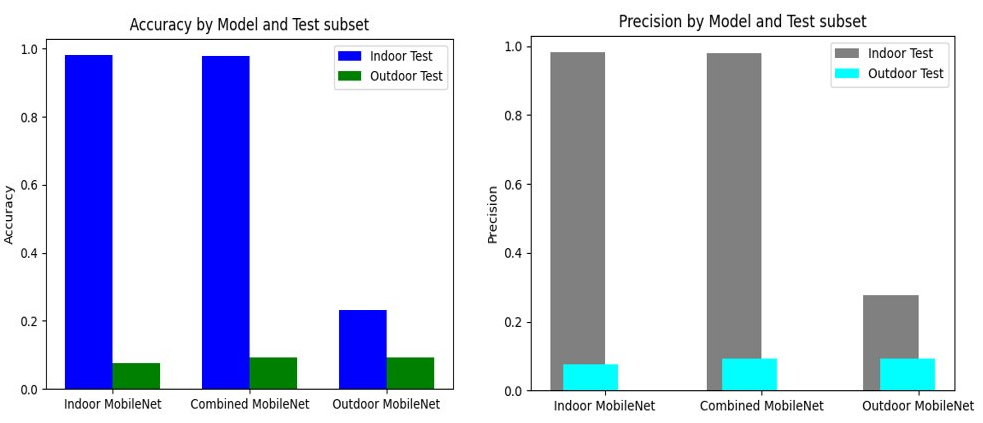
\includegraphics[width=8.5cm]{resultsPrecAccdifferentTests.png}}
\caption{Accuracy and Precision for the three models and tested on the indoors and outdoors test subsets.}
\label{fig}
\end{figure}
Of the models trained on the indoor, outdoor and combined data for the indoor test set the best performance was obtained with the indoor model with an accuracy of 98.1\%, as shown in figure. 8. The performance of the combined model gives similar accuracy of 98.0\%. The performance of the outdoor model in classifying the indoor test data is poor with an accuracy of 23.3\%. For the outdoor test set both the outdoor and combined models give the best classification performance with an accuracy of 9.2\%.The model trained on indoor data gives an accuracy of 7.5\% for the outdoor test set. From this we can see that for convolutional neural network models to be useful in detecting plant disease in real environments images of leaves taken outdoors should be used in training the models. \

For all three models the classification performance on the outdoor test set is poor. Considering there are 13 classes one would expect a random classifier to give an accuracy of 7.7\%. This poor performance may be due to the limited number of images in the outdoor test set which contains 120 images in total. \

\begin{figure}[htbp]
\centerline{\includegraphics[width=8cm]{indoor_images.png}}
\caption{Sample images left belongs to the Outdoor test and the right to the indoor test subset.}
\label{fig}
\end{figure}
In Fig. 9 a sample of images from the PlantVillage dataset for the thirteen classes considered in this study are shown. All images are taken in laboratory conditions with a similar plain background. \

In Fig.10 a sample of images based on images from the Plant Doc dataset for the thirteen classes considered in this study are shown. Various transformations have been applied to the original images for the purpose of augmentation. The original images were taken outdoors in real environments. 
\begin{figure}[htbp]
\centerline{\includegraphics[width=8.cm]{outdoor_images.png}}
\caption{Sample images left belongs to the Outdoor test and the right to the indoor test subset.}
\label{fig}
\end{figure}


\section{Conclusion and Future Work}

In this study it was shown that the models trained and tested using images produced in a controlled environment, in this case the laboratory, with consistent light and subject size produced satisfactory results, either the original coloured and the segmented images with different transfer functions (MobileNet and InceptionResNet). The size of the data set was large enough to guarantee good performance. On the other hand, the limitations in size of the data set in the case of the outdoor samples greatly diminished the accuracy of the models extracted from the sample. It was observed that there was not any gain by combining the two data sets in terms of performance over the outdoor test subset. It can be argued that combining both data sets to create a model that does not perform better than the models obtained from individual data sets is not efficient, as the resources needed are significantly larger without significant improvement. It has been shown that the biggest limitation to a successfully performing model is the quality and size of the data sets \

The lack of availability of images of leaves of diseased plants obtained outdoors in real world environments limited this study.  Given the disparity in quality of outdoor images, pictures are taken from different distances, different exposures, light, and they are generally inconsistent. A larger dataset of outdoor images would be required to be able to produce a successful model for leaf disease classification. Also, in this study only three plant species were considered. In future work classification of plant disease from images could be extended to include additional plant species.\

This study could be extended in a number of ways including through transfer learning using other pretrained CNN models to carry out image classification. In addition to the data augmentation techniques applied in this study other techniques could also be used including creating synthetic images of plant leaves using conditional generative adversarial networks. The Plant Doc outdoor images of leaves could be segmented and models, trained using these segmented images, compared against those trained using coloured versions of those images. We could extend this study from classifying the disease from the image of the leaf to grading how diseased the leaf is. In addition, we could compare the classification performance of the CNN models with that of other machine learning techniques. Our model could also be included as part of a pesticide prescription system for plant diseases. We could also compare the performance of a CNN model trained from scratch for classifying plant disease from leaf images against that of a CNN model trained by transfer learning. Our model could be used as part of a system to classify plant disease from images obtained using unmanned aerial vehicles. We could develop a lightweight model for devices with limited resources that still provides accurate performance in classifying plant disease from leaf images. The effect of varying the number of images used to train the models on the accuracy of classification could be investigated in future work.         


\bibliographystyle{IEEEtran}
\bibliography{references}

\end{document}
